\chapter{Computing Teaching Workload}
\label{ch:teaching_workload}

\section{Introduction}

The first step towards an equitable course allocation is to quantify the workload involved in teaching a course. Existing research shows that failing to accurately quantify this workload leads to considerable faculty dissatisfaction \cite{watts2011burnout}. Thus, accuracy and comprehensiveness of the workload calculation are essential, ensuring that the primary activities involved in teaching a course are accounted for, providing the faculty with an appropriate amount of time to perform each of these activities adequately.

Many previous attempts at computing the teaching workload have been retrospective, quantifying the course workload for analytic purposes. For course allocation, however, a prospective approach is required, computing the teaching workload as a function of the activities that need to be performed and the factors that affect them.

\textit{Griffith et al.} proposed a prospective approach, classifying the teaching workload into preparation, delivery, and grading \cite{griffith2020framework}. This research proposes a technique that builds upon this approach, adding additional granularity to more accurately account for the different types of teaching activity - lectures, tutorials, and labs.

Additionally, various factors are analyzed, and their impact on the teaching workload is incorporated into the technique. These factors are class size - which has a significant impact on the grading workload; faculty familiarity with the course material - which has a significant impact on the preparation workload; and type of teaching activity - which identifies the responsibilities of the faculty.

In the following sections, these components of course workload, and the factors affecting them are discussed in detail. The workload calculation technique is then demonstrated with real-world examples.

\section{Components of Teaching Workload}

For any given teaching activity assigned to a faculty, the teaching workload can be divided into multiple activities. These include preparing the course material before the course begins, reviewing and delivering the course material during the course, and grading the examinations and assignments during and after the course. These activities are described in the following sections.

\begin{enumerate}
  \item \textbf{Preparation (\(T_p\))} \\
        At the start of the semester, the faculty is assigned to teach a set of courses. Between the start of the semester and the first week of teaching, the faculty needs to prepare the course material for the course. The faculty has to spend a considerable amount of time researching and preparing the course material which involves designing up-to-date content for the course, time spent designing slides for the course, time spent designing an evaluation strategy for the course and accordingly, defining the rubric for the course and designing the examinations and assignments.

  \item \textbf{Pre-delivery Review (\(T_r\))} \\
        Before the delivery of each lecture, tutorial, or lab, the faculty needs to review the course material to refresh their understanding of the course material. This involves reviewing the lecture slides, reviewing the tutorial questions and solutions, and reviewing the lab experiments and solutions respectively. This can be a considerable amount of effort, especially for lectures, as the faculty needs to ensure the pace of the lecture is appropriate to complete the lecture materials, and the lecture is engaging.

  \item \textbf{Delivery (\(T_d\))} \\
        This refers to the contact time of the faculty with the students i.e. delivering the lectures or tutorials, or supervising the lab sessions. The faculty needs to ensure the comprehension and engagement of the students and engage in real-time feedback to adjust the pace of the lecture.

  \item \textbf{Grading (\(T_g\))} \\
        During the duration of the course, the faculty is responsible for grading the examinations and assignments. This includes grading the mid-semester exams, final exams, and any additional assignments that may be given. If the faculty is handling tutorial or lab sessions, they are also responsible for grading the tutorial assignments and lab reports.

        Since the preparation of examination material and the grading strategy is already done, this activity is largely clerical in nature. However, since this activity needs to be done individually for each student enrolled in the course, it can be a considerable amount of effort, especially for courses with a large number of students.

        Some assistance may be provided by teaching assistants in grading the examinations and assignments, but the faculty is primarily responsible for grading the examinations and assignments.

\end{enumerate}

In addition to the above activities, the faculty is also responsible for consultation hours, consolidation and entry of grades, as well as collection of teaching feedback from the students. However, these activities are not significant enough to affect the workload distribution and thus are not considered separately.

\section{Factors Affecting Teaching Workload}

Even for courses in the same study program or field, the teaching workload can vary significantly. This is because the teaching workload is affected by various factors.

First and foremost, the activity that is assigned to the faculty dictates the amount of workload the faculty has to handle. For example, if the faculty is assigned to deliver the lectures, their workload is naturally higher due to the additional responsibilities of preparing the lecture material and grading the examinations and assignments. However, if a faculty is assigned to deliver the tutorial or the lab session, they have no responsibility for preparing the course material, and thus the preparation workload is not considered. They also have a minimal grading workload, since the tutorial assignments and lab experiments are graded as part of the delivery of tutorials or lab respectively.

Course newness i.e. the familiarity of the faculty with the course material can have an impact on the teaching workload. If the faculty is unfamiliar with the course material, they will need to spend more time preparing the course material. However, other activities like delivering the lectures and grading the examinations and assignments are not affected by the course newness.

Class size also has a significant impact on grading workload \( T_g \), because the examinations and assignments need to be graded individually for each student enrolled in the course. However, the class size has minimal impact on the preparation of course material and delivery of lectures.

In the following sections, we will discuss the various factors that affect the teaching workload.

\subsection{Teaching Activity Type}
\label{sec:activity_type}

The workload of the faculty is directly affected by the activity that is assigned to them. A faculty assigned to deliver the lectures has a significantly higher workload than a faculty assigned to deliver the tutorials or labs.

If the faculty is assigned to deliver the lectures, they are responsible for preparing the course material for the lecture, the tutorial as well as the lab sessions. They also take the primary responsibility of grading the examinations and assignments. Thus, the workload of the faculty is significantly higher.

If the faculty is assigned to deliver the tutorials, they are not responsible for preparing the tutorial materials since the lecturer has already prepared the tutorial materials. They are responsible for reviewing the tutorial material before the tutorial session, and then delivering the tutorial session. Although they are also responsible for grading the tutorial assignments, this is largely done as part of the delivery of tutorials and thus doesn't need to be separately accounted for. Thus, the workload of the faculty is significantly lower.

Similarly, if the faculty is assigned to deliver the labs, they are not responsible for preparing the lab materials. They are responsible for reviewing the lab material before the lab session, and then delivering the lab session. Similar to tutorials, they are also responsible for grading the lab reports, but this is largely done as part of the delivery of labs, and thus doesn't need to be separately accounted for. Thus, the workload of the faculty is quite low as well.

\subsection{Course Newness}

The course newness is the familiarity of the faculty with the course material. Typically, the same course is taught by the same faculty every year, due to their prior experience with the course material. However, in a university with a large number of courses, it is fairly common for faculty to teach courses that they have not taught before due to the unavailability of other faculty. Additionally, fields with rapidly changing technology like Computer Science and Engineering require the introduction of new courses every year. Thus, the course newness can vary significantly between different courses.

The course newness primarily has an impact on the preparation of course material. If the faculty is unfamiliar with the course material, they will need to spend more time researching and preparing the course material. There might be cases where the faculty has not taught the course before, but another faculty has. In such cases, the course material prepared by the other faculty is readily available, and thus the preparation workload is reduced. Thus, course newness can have a significant impact on the preparation workload.

It can be argued that the course newness can have an impact on the delivery of lectures since new courses require additional preparation for the delivery of lectures. However, it can be assumed that the faculty already familiarized themselves with the course material during the preparation of course material, and thus the impact of such factors is assumed to be minimal.

Similarly, it can be argued that the course newness can have an impact on the grading of examinations and assignments since a new course would have varied responses from students. However, it is assumed that the examination material design and grading strategy are already prepared thoroughly to the extent that the grading workload is clerical in nature, and thus the impact of such factors is assumed to be minimal.

\subsection{Class Size}

The class size, i.e. the number of students enrolled in a course, can vary significantly between different courses. For example, a foundational course like Data Structures and Algorithms can have as many as 900 students enrolled in it, while an advanced course like Artificial Intelligence in Game Design can have as few as 30 students enrolled in it.

The class size has a significant impact on the grading workload. This is because the examinations and assignments need to be graded individually for each student enrolled in the course. Thus, the grading workload is directly proportional to the number of students enrolled in the course.

It can be argued that the class size can have an impact on the preparation of course material, since ensuring comprehension and engagement of the students can be more difficult for a larger class size, and the preparation of course materials needs to be more thorough. However, the impact of such factors is assumed to be minimal. Similar arguments made for the impact of class size on the delivery of lectures can also be ignored for the same reason.


\subsection{Factors With Minimal Impact}

Some other factors are important to consider, but their impact on the teaching workload was found to be minimal. This includes course complexity and faculty expertise. These factors are as follows:

\begin{itemize}
  \item  \textbf{Course Complexity}

        For latter-year specialization courses, the course material can be significantly more complex than foundational courses, and may also require more frequent updates. Course complexity can also vary depending on the field of study. For example, courses in fields with rapidly changing technology like Artificial Intelligence require more frequent updates to include state-of-the-art research in the corresponding fields. Thus, the course complexity can vary significantly between different courses.

        However, it is important to remember that faculty performs a significant amount of research as part of their job, and can be considered experts in their field of study. Since the faculty is typically assigned to teach a course according to their expertise, it can be assumed that the faculty is competent at teaching the course. Thus, the course complexity is assumed to have minimal impact on the teaching workload.

  \item \textbf{Mode of Delivery}

        There are various arguments arguing for a higher or lower workload for online courses compared to offline courses. The online mode of delivery can be argued to have a higher workload since the faculty needs to ensure that the students are engaged and comprehending the course material. However, the online mode of delivery can also be argued to have a lower workload since the faculty doesn't need to travel to the university to deliver the lectures.

        Through a survey of faculty, it was found that online delivery of lectures has a largely similar workload to offline delivery of lectures, with various factors contributing to an increase and decrease in workload. Thus, the mode of delivery is assumed to have a negligible impact on the teaching workload.

\end{itemize}

\begin{table}[htbp]
  \centering
  \begin{tabular}{|l|l|l|l|}
    \hline
    \textbf{Component}    & \textbf{Activity Type} & \textbf{Class Size}      & \textbf{Newness}         \\ \hline
    \(T_p\) - Preparation & Lecture                & -                        & \checkmark               \\
    \(T_r\) - Review      &                        & -                        & \checkmark               \\
    \(T_d\) - Delivery    &                        & -                        & -                        \\
    \(T_g\) - Grading     &                        & \checkmark               & -                        \\ \hline
    \(T_p\) - Preparation & Tutorial               & \textit{\color{gray}N/A} & \textit{\color{gray}N/A} \\
    \(T_r\) - Review      &                        & -                        & \checkmark               \\
    \(T_d\) - Delivery    &                        & -                        & -                        \\
    \(T_g\) - Grading     &                        & \textit{\color{gray}N/A} & \textit{\color{gray}N/A} \\ \hline
    \(T_p\) - Preparation & Lab Session            & \textit{\color{gray}N/A} & \textit{\color{gray}N/A} \\
    \(T_r\) - Review      &                        & -                        & \checkmark               \\
    \(T_d\) - Delivery    &                        & -                        & -                        \\
    \(T_g\) - Grading     &                        & \textit{\color{gray}N/A} & \textit{\color{gray}N/A} \\ \hline
  \end{tabular}
  \caption{Various factors and their impact on teaching workload}
  \label{tab:impact_on_teaching_workload_components}
\end{table}

\autoref{tab:impact_on_teaching_workload_components} describes the various factors that affect the teaching workload and how they impact the teaching workload. For lectures, the preparation and review workload is affected by the course newness, while the grading workload is affected by the class size. The delivery workload of the lecture is not affected by any of the factors.

For tutorials and labs, the preparation workload is not considered since the lecturer is responsible for preparing the tutorial and lab materials, as discussed in \autoref{sec:activity_type}. The review workload is affected by the course newness, since the faculty needs to spend more time reviewing the course material if they are unfamiliar with the course material. The delivery workload of tutorials and labs is not affected by any of the factors. The grading workload is also not considered since the grading of tutorial assignments and lab reports is largely done as part of the delivery of tutorials and labs respectively.


\section{Computing Lecture Workload}

Lecturing has the highest workload of all teaching activities since the lecturer for the course takes the primary responsibility of managing the course. This involves four primary activities - preparing the course material, reviewing and delivering the course material, and grading the examinations and assignments.

Preparation of course material involves a significant amount of research and preparation, designing up-to-date contents for the course, time spent designing lecture slides, time spent designing an evaluation strategy for the course and accordingly, defining the rubric for the course and designing the examinations and assignments. Additionally, even though tutorials and lab sessions are delivered by tutors and lab instructors respectively, the course lecturer has a significant role in preparing the tutorial and lab material. This includes designing the tutorial material and lab experiments, as well as the solutions to the tutorial and lab questions.

Reviewing the lecture material involves reviewing the lecture slides, and devising an approach to deliver the lecture material. The faculty needs to ensure the pace of the lecture is appropriate to complete the lecture materials, while also ensuring that the lecture is engaging. This takes a considerable amount of effort, given the large amount of course material that is typically covered in a lecture.

Delivering the lecture involves delivering the lecture material, ensuring comprehension and engagement of the students, and engaging in real-time feedback to adjust the pace of the lecture. Since the planning and preparation of the lecture material is already done, the faculty need only spend the classroom contact hours to deliver the lecture. Therefore, the delivery workload is lower than the preparation and review workloads.

Lastly, grading the examinations and assignments involves grading the mid-semester exams, final exams, and any additional assignments that may be given. This is largely clerical since the examination material design and grading strategy are already prepared. However, since this activity needs to be done individually for each student enrolled in the course, it can be a considerable amount of effort for courses with a large number of students.

\subsection{Course Material Preparation (\texorpdfstring{\(T_p\)}{})}
\label{sec:preparation_of_course_material}

As previously discussed, the preparation workload is affected by the course newness, while it is not affected by the class size. Thus, we can define the preparation workload as a function of the number of hours of lectures, tutorials, and labs, and the course newness.

First and foremost, the preparation workload is affected by the number of hours of lectures, tutorials, and labs. This is because for a longer lecture, the amount of course material that needs to be prepared proportionally increases. Similarly, for a longer tutorial or lab session, the amount of tutorial or lab material that needs to be prepared proportionally increases. Thus, the preparation workload is directly proportional to the number of hours of lectures, tutorials, and labs. it was found that for a completely new course:

\begin{itemize}
  \item \textbf{Preparation of lecture materials}

        The faculty needs to spend a significant amount of time researching and preparing the course material, which involves designing up-to-date content for the course, time spent designing lecture slides, time spent designing an evaluation strategy for the course and accordingly, defining the rubric for the course and designing the examinations and assignments. Since the lectures are the primary mode of delivery of the course material, the preparation of lecture materials essentially involves designing the contents and approach to the course. Thus, the preparation workload is the highest for lectures and was estimated to take 8 hours per hour of lecture.


  \item \textbf{Preparation of tutorial materials}

        Tutorials are typically 1 hour long, and the tutorial materials include supplementary material that expands on the lecture material, as well as tutorial questions and solutions and the assessment strategy for the tutorial. Since the tutorials are designed to be more interactive and engaging, the amount of course material that needs to be prepared is less than the amount of course material that needs to be prepared for lectures, which reduces the workload. Thus, the preparation workload is typically half of the preparation workload for lectures and was estimated to take 4 hours per hour of tutorial.

  \item \textbf{Preparation of lab materials}

        Labs are typically 2 hours long, and the lab materials include experiments that provide hands-on experience to the students, as well as lab questions and solutions and the assessment strategy for the lab. Since the labs focus on providing practical experience and an opportunity for self-learning, they require the least amount of involvement from the faculty. Thus, the material that needs to be prepared for labs is the least, which reduces the workload. Thus, preparing the lab materials for a 2-hour lab was estimated to take the same amount of time as preparing the tutorial materials for a 1-hour tutorial i.e. 2 hours per hour of lab.
\end{itemize}


Given the above correlation between the preparation workload and the number of hours of lectures, tutorials, and labs, we can define the preparation workload as a function of the number of hours of lectures, tutorials, and labs. So for a new course, the preparation workload is given by:

\begin{equation*}
  \label{eqn:preparation-workload}
  \begin{aligned}
    T_p^{lec} & = 8\ H^{lec} \\
    T_p^{tut} & = 4\ H^{tut} \\
    T_p^{lab} & = 2\ H^{lab}
  \end{aligned}
\end{equation*}

where \(T_p^{lec}\), \(T_p^{tut}\), and \(T_p^{lab}\) are the preparation workload for lecture, tutorial, and lab respectively, and \(H^{lec}\), \(H^{tut}\), and \(H^{lab}\) are the number of hours of lectures, tutorials, and labs respectively.

\subsubsection{Normalizing For Newness Using Newness Factors (\(N_1\) and \(N_2\))}

The familiarity of the faculty with the course material can have an impact on the preparation workload. If the faculty is unfamiliar with the course material, they will need to spend more time researching and preparing the course material. However, another faculty might have previously taught the same course, and thus the course material is readily available. Thus, the preparation workload can be divided into three distinct scenarios:

\begin{enumerate}
  \item \textbf{Course Coordinator has previously taught the course}\\
        If the course coordinator has previously taught the course, they only need to ensure that the course material is up to date. Thus, the time required to prepare the course material is negligible.

  \item \textbf{Course Coordinator has not previously taught the course, but another faculty has}\\
        If another faculty in the department has previously taught the course, the course material prepared by them is readily available. Most time is spent reviewing the course material and tailoring it to the course coordinator's teaching style. Thus, the time required to prepare the course material is moderate. Upon looking into previous cases of course preparation, it was found that the preparation workload is reduced by 60\% if another faculty has previously taught the course.

  \item \textbf{Course Coordinator has not previously taught the course, and no other faculty has either}\\
        If no other faculty in the department has previously taught the course, the course material needs to be prepared from scratch. This requires a significant amount of time and effort. Especially for advanced and novel courses, the research required to prepare the course material can be significant. Thus, the time required to prepare the course material is substantial.
\end{enumerate}

It was found that if another faculty has previously taught the course, the preparation workload is reduced by 60\%. It was also found that if the same course coordinator has previously taught the course, the preparation workload is negligible. To account for this, the \textbf{Newness to School} (\(N_1\)) and \textbf{Newness to Faculty} (\(N_2\)) factors were introduced. These factors are defined in \autoref{tab:n1-workload-factor} and \autoref{tab:n2-workload-factor} respectively.

\begin{table}[ht]
  \centering
  \begin{tabular}{|l|c|}
    \hline
    \textbf{Case}                 & \textbf{\(N_1\)} \\ \hline
    Course is new to school       & 1                \\ \hline
    Course has been taught before & 0.4              \\ \hline
  \end{tabular}
  \caption{\(N_1\) - Newness to School factor}
  \label{tab:n1-workload-factor}
\end{table}

\begin{table}[ht]
  \centering
  \begin{tabular}{|l|c|}
    \hline
    \textbf{Case}                        & \textbf{\(N_2\)} \\ \hline
    Course is new to Faculty             & 1                \\ \hline
    Faculty has taught the course before & 0                \\ \hline
  \end{tabular}
  \caption{\(N_2\) - Newness to Faculty factor}
  \label{tab:n2-workload-factor}
\end{table}

The need to introduce two separate factors is felt because, in certain scenarios, the workload of a course independent of the faculty needs to be known. For example, if the total workload for the school needs to be calculated, the workload of a course needs to be calculated independently of the faculty. In such a case, the \(N_1\) is used. However, if the workload of a faculty needs to be calculated, both \(N_1\) and \(N_2\) need to be considered.

For simplicity, we define the combined newness factor \(N = N_1 \times N_2\). Thus for the three cases of familiarity, the newness factors can be calculated as follows:

\begin{enumerate}
  \item Course is new to school and faculty has not taught the course before       \\
        \(N_1 = 1\) ; \(N_2 = 1\) ; \(N = 1\)
  \item Another faculty has taught the course before \\
        \(N_1 = 0.4\) ; \(N_2 = 1\) ; \(N = 0.4\)
  \item Course Coordinator has taught the course before     \\
        \(N_1 = 0.4\) ; \(N_2 = 0\) ; \(N = 0\)
\end{enumerate}

So, the preparation workload for a course is given by:

\begin{equation}
  \begin{aligned}
    T_p^{lec} & = 8   & \ N \ H^{lec} \\
    T_p^{tut} & = 5   & \ N \ H^{tut} \\
    T_p^{lab} & = 2.5 & \ N \ H^{lab}
  \end{aligned}
\end{equation}

In total, we can say

\begin{equation}
  \label{eqn:preparation-workload-total}
  \begin{aligned}
    T_p & = T_p^{lec} + T_p^{tut} + T_p^{lab}           \\
        & = N\ (8\ H^{lec} + 5\ H^{tut} + 2.5\ H^{lab})
  \end{aligned}
\end{equation}

\subsection{Lecture Review (\texorpdfstring{\(T_r^{lec}\)}{})}

Before the delivery of each lecture, the faculty needs to review the course material to refresh their understanding of the course material. This involves reviewing the lecture slides and devising an approach to deliver the lecture material. As previously discussed, the review workload is affected by the course newness, while it is not affected by the class size since the review workload is independent of the number of students enrolled in the course. Thus, we can define the review workload as a function of the number of hours of lectures and the course newness.

Firstly, the review workload is affected by the number of hours of lectures. This is because for a longer lecture, the amount of course material that needs to be reviewed and planned proportionally increases. Thus, the review workload is directly proportional to the number of hours of lectures. It was found that, for a completely new course, the review workload is 2 hours per hour of lecture. Given the above correlation between the review workload and the number of hours of lectures, we can define the review workload as a function of the number of hours of lectures. So for a new course, the review workload is given by:

\begin{equation*}
  \label{eqn:review-workload}
  T_r^{lec} = 2\ H^{lec}
\end{equation*}

Since the review workload is dependent on the course newness, we can use the newness factor \(N\) as defined in \autoref{sec:preparation_of_course_material}. This is because similar to the preparation workload, the review workload can also be assumed to drop to 40\% if another faculty has previously taught the course, and can be assumed to be negligible if the same course coordinator has previously taught the course. Thus, the review workload for a course is given by:

\begin{equation}
  \label{eqn:review-workload-total}
  T_r^{lec} = 2\ N \ H^{lec}
\end{equation}


\subsection{Lecture Delivery (\texorpdfstring{$T_d^{lec}$}{})}

Lecture delivery workload refers to the contact hours of the faculty with the students during the delivery of lectures. As previously discussed, the delivery workload is affected by neither the course newness nor the class size. Thus, we can define the delivery workload as a function of the number of hours of lectures.

It was found that since the preparation and review of lecture materials are already accounted for, the delivery workload can simply be defined as the number of hours of lectures. Therefore, the lecture delivery workload for a course is given by:

\begin{equation}
  \label{eqn:lecture-delivery-workload}
  T_d^{lec} = H^{lec}
\end{equation}

The lecture delivery workload is also inclusive of the time spent in consultation hours. However, consultation hours are usually minimal and thus, can be covered during the normal working hours of a faculty. Thus, the consultation workload is assumed to be insignificant and is not considered separately.

\subsection{Exam Grading (\texorpdfstring{\(T_g\)}{})}
\label{sec:exam_grading}

The exam grading workload is the time required to grade the exams - this includes grading the mid-semester exams, final exams, and any additional assignments that may be given. Although some assistance may be provided by teaching assistants, the faculty is primarily responsible for grading the exams.

As previously discussed, the exam grading workload is majorly affected by the class size, since the exam grading has to be done individually for each student enrolled in the course. Course newness does not have an impact on the exam grading workload, since the examination material design and grading strategy are already prepared, and thus the grading workload is the same for both new and old courses.

Given the above factors, we can define the exam grading workload as a function of the number of students enrolled in the course. Since the exam grading workload is directly proportional to the number of students enrolled in the course, the exam grading workload can be defined as a linear function of the number of students enrolled in the course. It was found that, on an aggregate, a faculty spends 2 hours per student per semester on grading. Thus, the exam grading workload for a course is given by:

\begin{equation*}
  \begin{aligned}
    T_g & = 2 S
  \end{aligned}
\end{equation*}
where \(S\) is the number of students enrolled in the course.

However, since the exam grading workload is clerical in nature, we need to account for the fact that an hour spent on grading is less taxing than an hour spent on teaching. Thus, a normalization factor is introduced to account for this.

\subsubsection{Normalizing For Cognitive Load Using Normalization Factor (\(N_g\))}

Not all teaching activities are equally taxing. For example, preparing the course material requires a significant amount of research, while correcting the examination papers is largely clerical in nature. Thus, the cognitive load associated with these activities can vary significantly. Although the amount of time spent in various teaching activities might be comparable, the cognitive load associated with some of the activities is significantly lower. Thus, we need to account for the cognitive load associated with each of these activities.

The cognitive effort associated with preparing the course material is significant, since it requires a significant amount of research and preparation, designing up-to-date content for the course, etc. Similarly, reviewing the course material also requires a significant amount of effort, since the faculty needs to ensure that they are familiar with the course material and the delivery of the lecture is well planned for. Delivering a lecture also requires a high amount of effort, since the faculty needs to ensure comprehension and engagement of the students, and engage in real-time feedback to adjust the pace of the lecture.

In comparison, grading the examinations and assignments is largely clerical in nature. The grading strategy is already prepared, and the faculty needs to simply apply the grading strategy to the examination papers. Thus, the cognitive load associated with grading the examinations and assignments is significantly lower than the cognitive load associated with preparing the course material, reviewing the course material, and delivering the lectures.

We need to incorporate the fact that an hour spent on grading is less taxing than an hour spent on teaching into our workload calculation. To account for this, a normalization factor \(N_g\) is introduced. It was found that faculty perceive the grading workload to be only 25\% effort in comparison to other teaching activities, i.e. 4 hours spent correcting examination papers is perceived to be a similar amount of effort as 1 hour spent delivering a lecture. Thus, we can say

\begin{equation*}
  \begin{aligned}
    N_g & = 0.25
  \end{aligned}
\end{equation*}


Thus, the exam grading workload can be defined as a function of the number of students enrolled in the course and the normalization factor \(N_g\) as:


\begin{equation}
  \label{eqn:exam-grading-workload}
  \begin{aligned}
    T_g & = N_g \times 2 \times S  \\
        & = 0.25 \times 2 \times S \\
    T_g & = 0.5\ S
  \end{aligned}
\end{equation}

\subsection{Holistic Lecture Workload Model}

The total workload for a course is the sum of the preparation workload, delivery workload, and exam grading workload. So, the total workload for the course coordinator is given by:

\begin{equation}
  \begin{aligned}
    T^{lec} & = T_p                                        & \ +\  & T_r            & \ +\  & T_d     & \ +\  & T_g    \\
            & = (8\ H^{lec} + 4\ H^{tut} + 2\ H^{lab})\ N  & \ +\  & 2\ N\  H^{lec} & \ +\  & H^{lec} & \ +\  & 0.5\ S \\
            & = (10\ H^{lec} + 4\ H^{tut} + 2\ H^{lab})\ N &       &                & \ +\  & H^{lec} & \ +\  & 0.5\ S \\
  \end{aligned}
\end{equation}
where,
\begin{equation*}
  \begin{aligned}
    N       & = newness\ factor                     \\
    H^{lec} & = hours\ of\ lectures                 \\
    H^{tut} & = hours\ of\ tutorials                \\
    H^{lab} & = hours\ of\ labs                     \\
    S       & = students\ enrolled\ in\ the\ course
  \end{aligned}
\end{equation*}

\section{Overcoming Major Deviations to Lecture Workload}

With the above definitions, we can now compute the workload for a course lecturer. As seen above, the workload for a course lecturer is a function of the number of hours of lectures, tutorials, and labs, the number of students enrolled in the course, and the newness of the course. However, the workload for a course lecturer can be disproportionately high for certain courses. This can be seen in the following examples:

\begin{table}[ht]
  \centering
  \begin{tabular}{|l|c|c|c|c|c|}
    \hline
    \textbf{Course}                        & \(H^{lec}\) & \(H^{tut}\) & \(H^{lab}\) & \(S\) & \(N\) \\\hline
    Computer Organisation \& Architecture  & 26          & 13          & 26          & 720   & 0.4   \\\hline
    Artificial Intelligence in Game Design & 39          & 0           & 0           & 26    & 0.4   \\\hline
    Data Structures                        & 26          & 13          & 26          & 25    & 1     \\\hline
  \end{tabular}
\end{table}

For the above examples, the lecture workload for the course coordinator is

\begin{enumerate}
  \item For Computer Organisation \& Architecture, the lecture workload is 532 units.
  \item For Artificial Intelligence in Game Design, the lecture workload is 208 units.
  \item For Data Structures, the lecture workload is 403 units.
\end{enumerate}

As can be seen, the workload for Computer Organisation and architecture is more than 2.5 times the workload of Artificial Intelligence in Game Design. Similarly, the workload for Data Structures is nearly 2 times the workload of Artificial Intelligence in Game Design. This is due to their higher class size and course newness respectively. This can lead to issues in maintaining an equitable workload distribution. These issues and remediation strategies are discussed in the following section.

\subsection{Problems with Workload Deviations}

A lecture with a disproportionately high workload in comparison to other lectures can lead to issues in maintaining an equitable workload distribution in multiple ways. Some of these issues are discussed below:

\begin{enumerate}

  \item \textbf{Research Active Faculty}

        A faculty with a high research workload might not have the bandwidth to teach a course with a high teaching workload. As a result, even if a faculty has expertise in a particular course's subject matter, they might not be able to teach the course due to a lack of bandwidth. They will instead be allocated a course with a lower teaching workload, which might not be in their area of expertise. This can lead to a sub-optimal allocation of courses.

  \item \textbf{Foundational Courses}

        Foundational courses like Data Structures and Algorithms, Computer Organisation and Architecture, etc. are required by multiple programs. As a result, these courses have a high number of students enrolled in them. However, the inability to allocate an experienced faculty to teach these courses can lead to sub-optimal learning outcomes for the students which can have a cascading effect on the students' performance in subsequent courses.

  \item \textbf{Inefficiencies in Allocating Multiple Courses}

        If a faculty is allocated a course with a high workload, it becomes difficult to allocate a second course to the faculty. This is because the workload of the faculty is already high, and allocating a second course can lead to an unfairly high workload for the faculty. On the other hand, if they're not allocated a second course, the faculty is underutilized, as well as creating supply-demand mismatches in the allocation of courses.

\end{enumerate}

\subsection{Course Mirroring}

For certain courses, the number of enrolled students is so high that a single lecture theatre is not enough to accommodate all the students. In such cases, the course is split into two separate sub-courses that are taught in two separate lecture theatres. Mirroring of courses into these sub-courses is done before the semester starts, as part of the course planning process taken up by the school. These sub-courses can therefore be treated as two separate courses for the purposes of the workload allocation process.  These sub-courses may be taught by the same faculty, or by different faculty. The sub-courses can also be staggered over the span of two semesters.


\subsection{Lecture Splitting}
\label{sec:lecture_splitting}

A way to pre-empt such workload inequities is to split the lecture workload of such courses between two or more faculty, which ensures that all faculty have a comparable workload. This process of splitting the workload of a course between two or more faculty is called \textbf{Lecture Splitting}.

When a lecture is split, additional course lecturers may be assigned and the responsibility of delivering the course is split into equal durations of the term. For example, if a 13-week course is taught by
2 course lecturers then they will be responsible for delivering the course for 7 and 6 weeks respectively. They also share equal responsibility for preparing the course material as well as designing the examinations and assignments for their respective parts and splitting the workload of grading the examinations equally.

The current practice is to split the workload of a course if the number of students enrolled in it exceeds certain thresholds. For example, if more than 200 students enrolled in a course, the course is split between two faculty. The rationale behind this is that in addition to being an indicator of the effort required to teach the course, the number of students is also a limiting factor as the number of halls big enough to accommodate such a large number of students is limited. However, this is not a good strategy as it does not take into account other factors that affect the workload. For example, a course with 200 students and 1 hour of lectures per week will have a lower workload than a new course with 100 students and 3 hours of lectures per week.

Since the workload of a course can be high due to other factors as well, the workload of a course is a better indicator of the effort required to teach the course. Thus, the workload of a course should be used as the primary indicator to split the workload of a course. For this purpose, thresholds of 300 and 500 workload units were set. If the workload of a course exceeds 300 units, the course is split between two faculty, and if it exceeds 500 units, the course is split between three faculty. This ensures that the total workload of a split course remains within a reasonable range.

It is important to note that the tutorial and lab workloads are already split into groups of 30-40 students and, as a result, do not need to be split further. Thus, as long as a reasonable number of tutorial and lab groups are allocated to each faculty, the tutorial and lab workload distribution remains fair.

\section{Computing Tutorial Workload}

Tutorials are supplementary sessions that are conducted to provide additional support to students and to provide an opportunity for students to engage with the course material. This includes solving any doubts that the students might have, as well as providing additional material that expands on the lecture material. Tutorials are typically 1 hour long and are conducted in groups of 30-40 students to ensure that the students have an opportunity to engage with the faculty.

Ideally, the lecturer and the tutor for a course are the same person, as this ensures that the students have a consistent experience across lectures and tutorials. However, this is not always possible due to the high workload of the lecturer. In such cases, the tutorial sessions are conducted by a separate faculty member called the tutor. The tutor is responsible for delivering the tutorial sessions, as well as grading the tutorial assignments.

Since the course materials for the tutorial sessions are already prepared by the lecturer, the preparation workload \(T_p\) is assumed to be negligible. Additionally, grading of tutorial assignments, although an important activity, is largely carried out as part of the delivery of materials, and thus doesn't need to be separately accounted for. Thus, the grading workload \(T_g\) is assumed to be negligible as well. Thus, the tutorial workload is primarily the review workload \(T_r\) and the delivery workload \(T_d\).

\subsection{Tutorial Review (\texorpdfstring{\(T_r^{tut}\)}{})}

Before the delivery of each tutorial, the faculty needs to review the materials that have been taught in the lecture. Additionally, the faculty needs to review the tutorial questions and solutions and devise an approach to deliver the tutorial material. This workload is referred to as the Tutorial Materials Review Workload (\(T_r^{tut}\)).

As previously discussed, the review workload is affected by the course newness, since a new course requires more time to review the course material in comparison to a course they have previously taught. On the other hand, the class size does not have an impact on the review workload, since the review workload is independent of the number of students enrolled in the course, and the number of students is approximately the same for all tutorial groups. Thus, we can define the review workload as a function of the number of hours of tutorials and the course newness.

For a new course, we found that for every hour of tutorial, a faculty spends approximately 2 hours reviewing the materials. Since the review workload is directly proportional to the number of hours of tutorials, the review workload can be defined as:

\begin{equation*}
  T_r^{tut} = 2\ H^{tut}
\end{equation*}

However, since the review workload is dependent on the course newness, we can use the newness factor \(N\) as defined in \autoref{sec:preparation_of_course_material}. This is because similar to the lecture review workload, the tutorial review workload can also be assumed to drop to 40\% if another faculty has previously taught the course, and can be assumed to be negligible if the same course coordinator has previously taught the course. Thus, the review workload for a course is given by:

\begin{equation}
  \label{eqn:tutorial-review-workload}
  T_r^{tut} = 2\ N \ H^{tut}
\end{equation}

\subsection{Tutorial Delivery (\texorpdfstring{\(T_d^{tut}\)}{})}

Tutorial delivery workload refers to the contact hours of the faculty with the students during the delivery of tutorials. As previously discussed, the delivery workload is affected by neither the course newness nor the class size. Thus, we can define the delivery workload as a function of the number of hours of tutorials.

It was found that since the preparation and review of tutorial materials are already accounted for, the delivery workload can simply be defined as the number of hours of tutorials. Therefore, the tutorial delivery workload for a course is given by:

\begin{equation}
  \label{eqn:tutorial-delivery-workload}
  T_d^{tut} = H^{tut}
\end{equation}

\subsection{Holistic Tutorial Workload Model (\texorpdfstring{\(T^{tut}\)}{})}

With the above definitions, we can now compute the workload for a course tutor. As seen above, the workload for a course tutor is a function of the number of hours of tutorials and the newness of the course. We can define the total tutorial workload as a sum of the review workload and the delivery workload. So, the total workload for the course tutor is given by:

\begin{equation}
  \begin{aligned}
    T^{tut} & = T_r^{tut}           & \ +\  & T_d^{tut} \\
            & = 2\ N\ H^{tut}       & \ +\  & H^{tut}   \\
            & = (2\ N + 1)\ H^{tut}
  \end{aligned}
  \label{eqn:tutorial-workload}
\end{equation}

Where, \(N\) is the newness factor as defined in \autoref{sec:preparation_of_course_material}, \(H^{tut}\) is the number of hours of tutorials, \(T_r^{tut}\) is the tutorial review workload, and \(T_d^{tut}\) is the tutorial delivery workload.

\section{Computing Lab Workload}

Labs are supplementary sessions that are conducted to provide hands-on experience to the students. A typical lab session consists of a lab experiment that provides hands-on experience to the students. The students might be graded on their performance in the lab experiment or might be required to submit a lab report. Labs are typically 2 hours long and are conducted in groups of 30-40 students to ensure that the students have an opportunity to engage with the faculty.

Similar to tutorials, the lecturer and the lab assistant for a course are ideally the same person. However, this is not always possible due to the high workload of the lecturer. In such cases, the lab sessions are conducted by a separate faculty member called the lab instructor. The lab instructor is responsible for delivering the lab sessions, as well as grading the lab reports.

Similar to tutorials, the preparation workload \(T_p\) is assumed to be negligible as the preparation of lab materials is already accounted for in the lecture preparation workload, and the grading workload \(T_g\) is assumed to be negligible as well since the grading of lab reports is typically done during the delivery of the lab sessions. Thus, the lab workload is primarily the review workload \(T_r\) and the delivery workload \(T_d\).

\subsection{Holistic Lab Workload Model (\texorpdfstring{\(T^{lab}\)}{})}

The lab workload is very similar in nature to the tutorial workload. Thus, we can define the total lab workload in a similar manner as the tutorial workload.

For a new course, we found that for every hour of lab, a faculty spends approximately 1 hour reviewing the materials. Similar to the tutorial workload, the lab workload is also dependent on the course newness. Thus, we can use the newness factor \(N\) as defined in \autoref{sec:preparation_of_course_material}. Thus, the review workload for a course is given by:

\begin{equation}
  \label{eqn:lab-review-workload}
  T_r^{lab} = 1\ N \ H^{lab}
\end{equation}

Similar to the tutorial workload, the lab delivery workload is also defined as the number of hours of labs. Therefore, the lab delivery workload for a course is given by:

\begin{equation}
  \label{eqn:lab-delivery-workload}
  T_d^{lab} = H^{lab}
\end{equation}

With the above definitions, we can now compute the total workload for a course lab instructor. As seen above, the workload for a course lab instructor is a function of the number of hours of labs and the newness of the course. We can define the total lab workload as a sum of the review workload and the delivery workload. So, the total workload for the course lab instructor is given by:

\begin{equation}
  \begin{aligned}
    T^{lab} & = T_r^{lab}        & \ +\  & T_d^{lab} \\
            & = 1\ N\ H^{lab}    & \ +\  & H^{lab}   \\
            & = (N + 1)\ H^{lab}
  \end{aligned}
  \label{eqn:lab-workload}
\end{equation}

Where, \(N\) is the newness factor as defined in \autoref{sec:preparation_of_course_material}, \(H^{lab}\) is the number of hours of labs, \(T_r^{lab}\) is the lab review workload, and \(T_d^{lab}\) is the lab delivery workload.

\section{Total Teaching Workload}

The total course workload is the sum of the tutorial, lab, and lecture workload. The total workload can be used as a comparative metric to determine the comparative workload of different courses, which can help to understand the workload distribution across courses, as well as estimate the need for course mirroring. The total workload can be calculated as follows:

\begin{equation}
  \label{eqn:total-course-workload}
  \begin{aligned}
    T & = T^{lec}                                                               & \ +\  & T^{tut}             & \ +\  & T^{lab}          \\
      & = (10\ H^{lec} + 4\ H^{tut} + 2\ H^{lab})\ N\ +\ H^{lec}  \ +\   0.5\ S & \ +\  & (2\ N + 1)\ H^{tut} & \ +\  & (N + 1)\ H^{lab} \\
      & = (10\ N + 1)H^{lec} + (6\ N + 1)H^{tut} + (3\ N + 1)H^{lab}            & \ +\  & 0.5\ S
  \end{aligned}
\end{equation}

where,
\begin{equation*}
  \nonumber
  \begin{aligned}
    N       & = newness\ factor                     \\
    H^{lec} & = hours\ of\ lectures                 \\
    H^{tut} & = hours\ of\ tutorials                \\
    H^{lab} & = hours\ of\ labs                     \\
    S       & = students\ enrolled\ in\ the\ course
  \end{aligned}
\end{equation*}

Other activities like consultation hours, office hours, and entry of grades and moderation are not included in the workload calculation because they are not significant enough to affect the workload distribution.

\begin{figure}[ht]
  \centering
  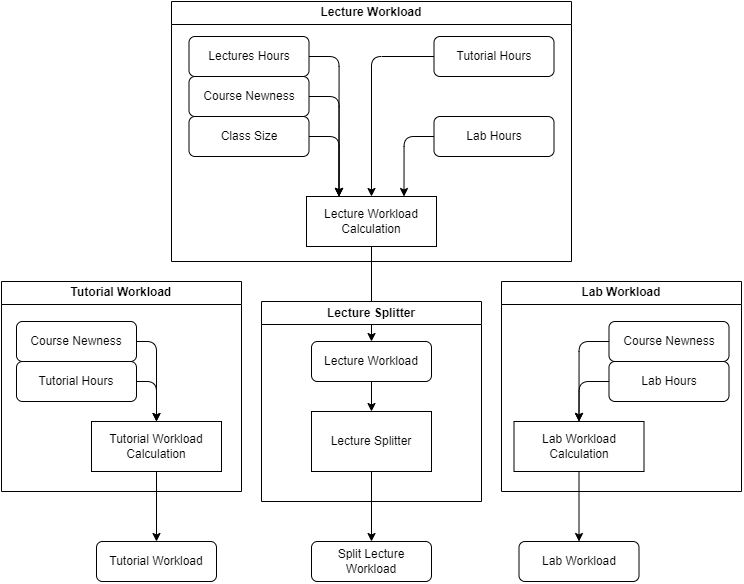
\includegraphics[width=0.9\textwidth]{images/teaching_workload.png}
  \caption{An overview of the teaching workload calculation process}
  \label{fig:teaching-workload}
\end{figure}

\autoref{fig:teaching-workload} shows an overview of the teaching workload calculation process. The workload calculation process is divided into lecture, tutorial, and lab workload calculation. The calculated lecture workload further passes through the lecture splitting process to provide the split lecture workload.


\subsection{Demonstration of the model}
\label{sec:workload_demo}

For the purposes of demonstration, we will consider three examples:

\begin{table}[ht]
  \centering
  \begin{tabular}{|l|c|c|c|c|c|}
    \hline
    \textbf{Course}                                  & \(H^{lec}\) & \(H^{tut}\) & \(H^{lab}\) & \(S\) & \(N\) \\\hline
    \(C_1\) - Computer Organisation \& Architecture  & 26          & 13          & 26          & 720   & 0.4   \\\hline
    \(C_2\) - Artificial Intelligence in Game Design & 39          & 0           & 0           & 26    & 0.4   \\\hline
    \(C_3\) - Data Structures                        & 26          & 13          & 26          & 25    & 1     \\\hline
  \end{tabular}
\end{table}

For the above examples, the course workload is shown to be:

\begin{table}[ht]
  \centering
  \begin{tabular}{|l|c|c|c|c|}
    \hline
    \textbf{Course}                                  & \(T_{total}\) & \(T^{lec}\) & \(T^{tut}\) & \(T^{lab}\) \\\hline
    \(C_1\) - Computer Organisation \& Architecture  & 591           & 532         & 23          & 36          \\\hline
    \(C_2\) - Artificial Intelligence in Game Design & 208           & 208         & 0           & 0           \\\hline
    \(C_3\) - Data Structures                        & 493           & 403         & 39          & 52          \\\hline
  \end{tabular}
\end{table}

As you can see, the workload for \(C_1\) is around 3 times the workload of \(C_2\). Most of the difference in workload is accounted for in the lecture workload (\(T_{lec}\)) since the lecture workload is the highest component of the total workload.

You can also see the difference in tutorial and lab workload between \(C_1\) and \(C_3\). This is due to the course newness factor, since \(C_3\) is a new course, while \(C_1\) is an old course. Even with this difference, the tutorial and lab workloads for the two courses are still comparable.

\section{Summary}

In this chapter, we discussed the teaching workload calculation process. We started by defining the various components of the teaching workload and then discussed the process of calculating the workload for each of these components. We also discussed the process of splitting the workload of a course between two or more faculty, and the process of mirroring a course into two or more sub-courses. Finally, we demonstrated the workload calculation process using three examples. This approach to calculating the teaching workload was found to be holistic and effective in calculating the workload for a course and will serve as the basis of teaching workload calculation.

In the next chapter, we will discuss the Faculty Workload Model, which aims to provide a clear and transparent picture of the workload of a faculty. The Faculty Workload Model is then used to calculate the teaching workload of a faculty, which will serve as the basis of the allocation process.
